% Created by tikzDevice version 0.12.3.1 on 2022-09-01 15:46:47
% !TEX encoding = UTF-8 Unicode
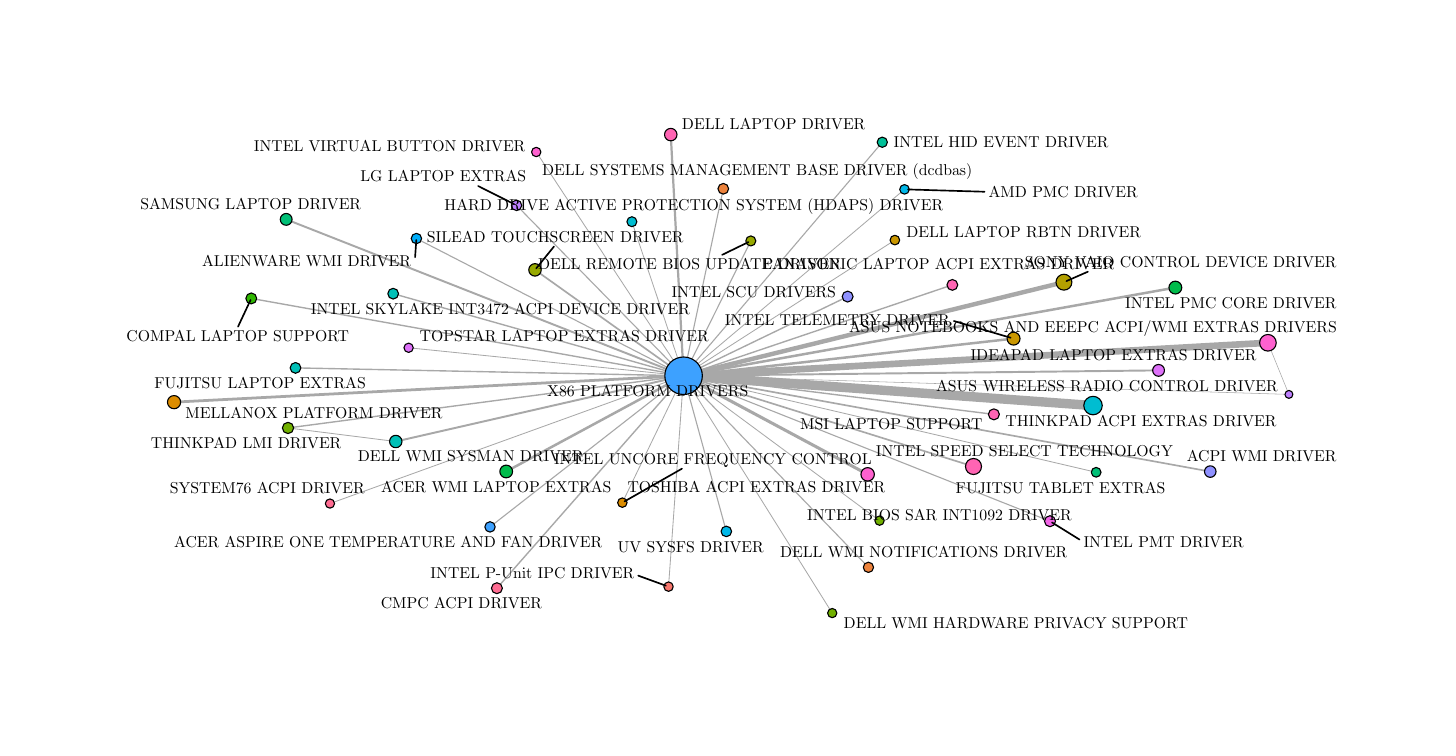
\begin{tikzpicture}[x=1pt,y=1pt]
\definecolor{fillColor}{RGB}{255,255,255}
\path[use as bounding box,fill=fillColor,fill opacity=0.00] (0,0) rectangle (505.89,252.94);
\begin{scope}
\path[clip] (  0.00,  0.00) rectangle (505.89,252.94);
\definecolor{fillColor}{RGB}{255,255,255}

\path[fill=fillColor] (  0.00,  0.00) rectangle (505.89,252.94);
\end{scope}
\begin{scope}
\path[clip] ( 32.75, 32.75) rectangle (475.89,222.94);
\definecolor{drawColor}{gray}{0.66}

\path[draw=drawColor,line width= 0.4pt,line join=round] (167.07, 72.54) -- (237.01,127.16);

\path[draw=drawColor,line width= 0.9pt,line join=round] (172.92, 92.57) -- (237.01,127.16);

\path[draw=drawColor,line width= 0.6pt,line join=round] (427.33, 92.53) -- (237.01,127.16);

\path[draw=drawColor,line width= 0.4pt,line join=round] (140.47,176.75) -- (237.01,127.16);

\path[draw=drawColor,line width= 0.3pt,line join=round] (316.84,194.51) -- (237.01,127.16);

\path[draw=drawColor,line width= 0.2pt,line join=round] (448.16,139.07) -- (455.75,120.42);

\path[draw=drawColor,line width= 2.4pt,line join=round] (448.16,139.07) -- (237.01,127.16);

\path[draw=drawColor,line width= 0.2pt,line join=round] (455.75,120.42) -- (237.01,127.16);

\path[draw=drawColor,line width= 0.5pt,line join=round] (169.56, 50.39) -- (237.01,127.16);

\path[draw=drawColor,line width= 0.5pt,line join=round] ( 80.80,155.10) -- (237.01,127.16);

\path[draw=drawColor,line width= 0.8pt,line join=round] (232.38,214.30) -- (237.01,127.16);

\path[draw=drawColor,line width= 0.3pt,line join=round] (313.36,176.18) -- (237.01,127.16);

\path[draw=drawColor,line width= 0.4pt,line join=round] (261.30,175.87) -- (237.01,127.16);

\path[draw=drawColor,line width= 0.4pt,line join=round] (251.36,194.72) -- (237.01,127.16);

\path[draw=drawColor,line width= 0.3pt,line join=round] (290.72, 41.40) -- (237.01,127.16);

\path[draw=drawColor,line width= 0.4pt,line join=round] (303.80, 57.94) -- (237.01,127.16);

\path[draw=drawColor,line width= 0.3pt,line join=round] (133.01,103.40) -- ( 94.07,108.30);

\path[draw=drawColor,line width= 0.7pt,line join=round] (133.01,103.40) -- (237.01,127.16);

\path[draw=drawColor,line width= 0.5pt,line join=round] ( 96.78,130.00) -- (237.01,127.16);

\path[draw=drawColor,line width= 0.3pt,line join=round] (386.09, 92.28) -- (237.01,127.16);

\path[draw=drawColor,line width= 0.3pt,line join=round] (218.33,182.82) -- (237.01,127.16);

\path[draw=drawColor,line width= 0.7pt,line join=round] (408.64,129.10) -- (237.01,127.16);

\path[draw=drawColor,line width= 0.3pt,line join=round] (307.82, 74.80) -- (237.01,127.16);

\path[draw=drawColor,line width= 0.4pt,line join=round] (308.81,211.54) -- (237.01,127.16);

\path[draw=drawColor,line width= 0.3pt,line join=round] (231.57, 50.95) -- (237.01,127.16);

\path[draw=drawColor,line width= 0.9pt,line join=round] (414.71,159.02) -- (237.01,127.16);

\path[draw=drawColor,line width= 0.4pt,line join=round] (369.41, 74.60) -- (237.01,127.16);

\path[draw=drawColor,line width= 0.5pt,line join=round] (296.29,155.77) -- (237.01,127.16);

\path[draw=drawColor,line width= 0.5pt,line join=round] (132.07,156.82) -- (237.01,127.16);

\path[draw=drawColor,line width= 0.6pt,line join=round] (341.77, 94.37) -- (237.01,127.16);

\path[draw=drawColor,line width= 0.9pt,line join=round] (356.25,140.58) -- (237.01,127.16);

\path[draw=drawColor,line width= 0.3pt,line join=round] (214.89, 81.31) -- (237.01,127.16);

\path[draw=drawColor,line width= 0.3pt,line join=round] (183.77,208.01) -- (237.01,127.16);

\path[draw=drawColor,line width= 0.4pt,line join=round] (176.64,188.74) -- (237.01,127.16);

\path[draw=drawColor,line width= 1.0pt,line join=round] ( 52.89,117.62) -- (237.01,127.16);

\path[draw=drawColor,line width= 0.5pt,line join=round] (349.14,113.21) -- (237.01,127.16);

\path[draw=drawColor,line width= 0.5pt,line join=round] (334.13,159.99) -- (237.01,127.16);

\path[draw=drawColor,line width= 0.7pt,line join=round] ( 93.41,183.67) -- (237.01,127.16);

\path[draw=drawColor,line width= 0.6pt,line join=round] (183.32,165.42) -- (237.01,127.16);

\path[draw=drawColor,line width= 1.6pt,line join=round] (374.45,160.97) -- (237.01,127.16);

\path[draw=drawColor,line width= 0.3pt,line join=round] (109.22, 80.98) -- (237.01,127.16);

\path[draw=drawColor,line width= 3.4pt,line join=round] (384.96,116.39) -- (237.01,127.16);

\path[draw=drawColor,line width= 0.5pt,line join=round] ( 94.07,108.30) -- (237.01,127.16);

\path[draw=drawColor,line width= 0.3pt,line join=round] (137.65,137.27) -- (237.01,127.16);

\path[draw=drawColor,line width= 1.1pt,line join=round] (303.52, 91.53) -- (237.01,127.16);

\path[draw=drawColor,line width= 0.4pt,line join=round] (252.46, 70.91) -- (237.01,127.16);
\definecolor{drawColor}{RGB}{0,0,0}
\definecolor{fillColor}{RGB}{61,161,255}

\path[draw=drawColor,line width= 0.4pt,line join=round,line cap=round,fill=fillColor] (167.07, 72.54) circle (  1.88);
\definecolor{fillColor}{RGB}{0,187,75}

\path[draw=drawColor,line width= 0.4pt,line join=round,line cap=round,fill=fillColor] (172.92, 92.57) circle (  2.30);
\definecolor{fillColor}{RGB}{143,145,255}

\path[draw=drawColor,line width= 0.4pt,line join=round,line cap=round,fill=fillColor] (427.33, 92.53) circle (  2.08);
\definecolor{fillColor}{RGB}{0,174,250}

\path[draw=drawColor,line width= 0.4pt,line join=round,line cap=round,fill=fillColor] (140.47,176.75) circle (  1.88);
\definecolor{fillColor}{RGB}{0,183,232}

\path[draw=drawColor,line width= 0.4pt,line join=round,line cap=round,fill=fillColor] (316.84,194.51) circle (  1.73);
\definecolor{fillColor}{RGB}{254,97,207}

\path[draw=drawColor,line width= 0.4pt,line join=round,line cap=round,fill=fillColor] (448.16,139.07) circle (  3.00);
\definecolor{fillColor}{RGB}{190,128,255}

\path[draw=drawColor,line width= 0.4pt,line join=round,line cap=round,fill=fillColor] (455.75,120.42) circle (  1.43);
\definecolor{fillColor}{RGB}{255,108,146}

\path[draw=drawColor,line width= 0.4pt,line join=round,line cap=round,fill=fillColor] (169.56, 50.39) circle (  1.98);
\definecolor{fillColor}{RGB}{47,182,0}

\path[draw=drawColor,line width= 0.4pt,line join=round,line cap=round,fill=fillColor] ( 80.80,155.10) circle (  1.97);
\definecolor{fillColor}{RGB}{255,100,179}

\path[draw=drawColor,line width= 0.4pt,line join=round,line cap=round,fill=fillColor] (232.38,214.30) circle (  2.25);
\definecolor{fillColor}{RGB}{202,151,0}

\path[draw=drawColor,line width= 0.4pt,line join=round,line cap=round,fill=fillColor] (313.36,176.18) circle (  1.74);
\definecolor{fillColor}{RGB}{151,169,0}

\path[draw=drawColor,line width= 0.4pt,line join=round,line cap=round,fill=fillColor] (261.30,175.87) circle (  1.82);
\definecolor{fillColor}{RGB}{236,130,60}

\path[draw=drawColor,line width= 0.4pt,line join=round,line cap=round,fill=fillColor] (251.36,194.72) circle (  1.93);
\definecolor{fillColor}{RGB}{113,176,0}

\path[draw=drawColor,line width= 0.4pt,line join=round,line cap=round,fill=fillColor] (290.72, 41.40) circle (  1.67);
\definecolor{fillColor}{RGB}{236,130,60}

\path[draw=drawColor,line width= 0.4pt,line join=round,line cap=round,fill=fillColor] (303.80, 57.94) circle (  1.86);
\definecolor{fillColor}{RGB}{0,192,183}

\path[draw=drawColor,line width= 0.4pt,line join=round,line cap=round,fill=fillColor] (133.01,103.40) circle (  2.24);

\path[draw=drawColor,line width= 0.4pt,line join=round,line cap=round,fill=fillColor] ( 96.78,130.00) circle (  1.94);
\definecolor{fillColor}{RGB}{0,191,118}

\path[draw=drawColor,line width= 0.4pt,line join=round,line cap=round,fill=fillColor] (386.09, 92.28) circle (  1.76);
\definecolor{fillColor}{RGB}{0,189,209}

\path[draw=drawColor,line width= 0.4pt,line join=round,line cap=round,fill=fillColor] (218.33,182.82) circle (  1.80);
\definecolor{fillColor}{RGB}{222,113,249}

\path[draw=drawColor,line width= 0.4pt,line join=round,line cap=round,fill=fillColor] (408.64,129.10) circle (  2.13);
\definecolor{fillColor}{RGB}{113,176,0}

\path[draw=drawColor,line width= 0.4pt,line join=round,line cap=round,fill=fillColor] (307.82, 74.80) circle (  1.69);
\definecolor{fillColor}{RGB}{0,192,152}

\path[draw=drawColor,line width= 0.4pt,line join=round,line cap=round,fill=fillColor] (308.81,211.54) circle (  1.85);
\definecolor{fillColor}{RGB}{248,118,109}

\path[draw=drawColor,line width= 0.4pt,line join=round,line cap=round,fill=fillColor] (231.57, 50.95) circle (  1.70);
\definecolor{fillColor}{RGB}{0,187,75}

\path[draw=drawColor,line width= 0.4pt,line join=round,line cap=round,fill=fillColor] (414.71,159.02) circle (  2.32);
\definecolor{fillColor}{RGB}{242,101,231}

\path[draw=drawColor,line width= 0.4pt,line join=round,line cap=round,fill=fillColor] (369.41, 74.60) circle (  1.99);
\definecolor{fillColor}{RGB}{143,145,255}

\path[draw=drawColor,line width= 0.4pt,line join=round,line cap=round,fill=fillColor] (296.29,155.77) circle (  1.97);
\definecolor{fillColor}{RGB}{0,192,183}

\path[draw=drawColor,line width= 0.4pt,line join=round,line cap=round,fill=fillColor] (132.07,156.82) circle (  1.94);
\definecolor{fillColor}{RGB}{255,100,179}

\path[draw=drawColor,line width= 0.4pt,line join=round,line cap=round,fill=fillColor] (341.77, 94.37) circle (  2.89);
\definecolor{fillColor}{RGB}{202,151,0}

\path[draw=drawColor,line width= 0.4pt,line join=round,line cap=round,fill=fillColor] (356.25,140.58) circle (  2.34);
\definecolor{fillColor}{RGB}{221,141,0}

\path[draw=drawColor,line width= 0.4pt,line join=round,line cap=round,fill=fillColor] (214.89, 81.31) circle (  1.71);
\definecolor{fillColor}{RGB}{254,97,207}

\path[draw=drawColor,line width= 0.4pt,line join=round,line cap=round,fill=fillColor] (183.77,208.01) circle (  1.69);
\definecolor{fillColor}{RGB}{190,128,255}

\path[draw=drawColor,line width= 0.4pt,line join=round,line cap=round,fill=fillColor] (176.64,188.74) circle (  1.89);
\definecolor{fillColor}{RGB}{221,141,0}

\path[draw=drawColor,line width= 0.4pt,line join=round,line cap=round,fill=fillColor] ( 52.89,117.62) circle (  2.38);
\definecolor{fillColor}{RGB}{255,100,179}

\path[draw=drawColor,line width= 0.4pt,line join=round,line cap=round,fill=fillColor] (349.14,113.21) circle (  1.99);

\path[draw=drawColor,line width= 0.4pt,line join=round,line cap=round,fill=fillColor] (334.13,159.99) circle (  1.95);
\definecolor{fillColor}{RGB}{0,191,118}

\path[draw=drawColor,line width= 0.4pt,line join=round,line cap=round,fill=fillColor] ( 93.41,183.67) circle (  2.13);
\definecolor{fillColor}{RGB}{151,169,0}

\path[draw=drawColor,line width= 0.4pt,line join=round,line cap=round,fill=fillColor] (183.32,165.42) circle (  2.25);
\definecolor{fillColor}{RGB}{179,160,0}

\path[draw=drawColor,line width= 0.4pt,line join=round,line cap=round,fill=fillColor] (374.45,160.97) circle (  2.87);
\definecolor{fillColor}{RGB}{255,108,146}

\path[draw=drawColor,line width= 0.4pt,line join=round,line cap=round,fill=fillColor] (109.22, 80.98) circle (  1.67);
\definecolor{fillColor}{RGB}{0,189,209}

\path[draw=drawColor,line width= 0.4pt,line join=round,line cap=round,fill=fillColor] (384.96,116.39) circle (  3.34);
\definecolor{fillColor}{RGB}{113,176,0}

\path[draw=drawColor,line width= 0.4pt,line join=round,line cap=round,fill=fillColor] ( 94.07,108.30) circle (  2.04);
\definecolor{fillColor}{RGB}{222,113,249}

\path[draw=drawColor,line width= 0.4pt,line join=round,line cap=round,fill=fillColor] (137.65,137.27) circle (  1.68);
\definecolor{fillColor}{RGB}{254,97,207}

\path[draw=drawColor,line width= 0.4pt,line join=round,line cap=round,fill=fillColor] (303.52, 91.53) circle (  2.43);
\definecolor{fillColor}{RGB}{0,183,232}

\path[draw=drawColor,line width= 0.4pt,line join=round,line cap=round,fill=fillColor] (252.46, 70.91) circle (  1.91);
\definecolor{fillColor}{RGB}{61,161,255}

\path[draw=drawColor,line width= 0.4pt,line join=round,line cap=round,fill=fillColor] (237.01,127.16) circle (  6.78);

\path[draw=drawColor,line width= 0.6pt,line join=round,line cap=round] (139.99,169.97) -- (140.43,176.21);

\path[draw=drawColor,line width= 0.6pt,line join=round,line cap=round] (345.79,193.65) -- (318.11,194.48);

\path[draw=drawColor,line width= 0.6pt,line join=round,line cap=round] ( 76.01,144.89) -- ( 80.55,154.56);

\path[draw=drawColor,line width= 0.6pt,line join=round,line cap=round] (250.95,170.85) -- (260.46,175.47);

\path[draw=drawColor,line width= 0.6pt,line join=round,line cap=round] (220.63, 54.93) -- (230.60, 51.30);

\path[draw=drawColor,line width= 0.6pt,line join=round,line cap=round] (380.08, 67.97) -- (370.13, 74.15);

\path[draw=drawColor,line width= 0.6pt,line join=round,line cap=round] (334.67,146.94) -- (355.20,140.89);

\path[draw=drawColor,line width= 0.6pt,line join=round,line cap=round] (236.42, 93.58) -- (215.66, 81.75);

\path[draw=drawColor,line width= 0.6pt,line join=round,line cap=round] (162.80,195.71) -- (175.82,189.15);

\path[draw=drawColor,line width= 0.6pt,line join=round,line cap=round] (190.17,173.85) -- (183.74,165.93);

\path[draw=drawColor,line width= 0.6pt,line join=round,line cap=round] (383.10,164.76) -- (375.34,161.36);

\node[text=drawColor,anchor=base,inner sep=0pt, outer sep=0pt, scale=  0.57] at (130.27, 65.09) {ACER ASPIRE ONE TEMPERATURE AND FAN DRIVER};

\node[text=drawColor,anchor=base,inner sep=0pt, outer sep=0pt, scale=  0.57] at (169.32, 85.07) {ACER WMI LAPTOP EXTRAS};

\node[text=drawColor,anchor=base,inner sep=0pt, outer sep=0pt, scale=  0.57] at (445.89, 96.10) {ACPI WMI DRIVER};

\node[text=drawColor,anchor=base,inner sep=0pt, outer sep=0pt, scale=  0.57] at (100.79,166.55) {ALIENWARE WMI DRIVER};

\node[text=drawColor,anchor=base,inner sep=0pt, outer sep=0pt, scale=  0.57] at (374.17,191.68) {AMD PMC DRIVER};

\node[text=drawColor,anchor=base,inner sep=0pt, outer sep=0pt, scale=  0.57] at (384.93,142.61) {ASUS NOTEBOOKS AND EEEPC ACPI/WMI EXTRAS DRIVERS};

\node[text=drawColor,anchor=base,inner sep=0pt, outer sep=0pt, scale=  0.57] at (390.00,121.61) {ASUS WIRELESS RADIO CONTROL DRIVER};

\node[text=drawColor,anchor=base,inner sep=0pt, outer sep=0pt, scale=  0.57] at (156.73, 42.93) {CMPC ACPI DRIVER};

\node[text=drawColor,anchor=base,inner sep=0pt, outer sep=0pt, scale=  0.57] at ( 75.91,139.47) {COMPAL LAPTOP SUPPORT};

\node[text=drawColor,anchor=base,inner sep=0pt, outer sep=0pt, scale=  0.57] at (269.56,216.00) {DELL LAPTOP DRIVER};

\node[text=drawColor,anchor=base,inner sep=0pt, outer sep=0pt, scale=  0.57] at (359.89,177.10) {DELL LAPTOP RBTN DRIVER};

\node[text=drawColor,anchor=base,inner sep=0pt, outer sep=0pt, scale=  0.57] at (239.16,165.42) {DELL REMOTE BIOS UPDATE DRIVER};

\node[text=drawColor,anchor=base,inner sep=0pt, outer sep=0pt, scale=  0.57] at (263.62,199.63) {DELL SYSTEMS MANAGEMENT BASE DRIVER (dcdbas)};

\node[text=drawColor,anchor=base,inner sep=0pt, outer sep=0pt, scale=  0.57] at (357.07, 35.76) {DELL WMI HARDWARE PRIVACY SUPPORT};

\node[text=drawColor,anchor=base,inner sep=0pt, outer sep=0pt, scale=  0.57] at (323.75, 61.50) {DELL WMI NOTIFICATIONS DRIVER};

\node[text=drawColor,anchor=base,inner sep=0pt, outer sep=0pt, scale=  0.57] at (160.08, 96.13) {DELL WMI SYSMAN DRIVER};

\node[text=drawColor,anchor=base,inner sep=0pt, outer sep=0pt, scale=  0.57] at ( 83.97,122.54) {FUJITSU LAPTOP EXTRAS};

\node[text=drawColor,anchor=base,inner sep=0pt, outer sep=0pt, scale=  0.57] at (373.23, 84.79) {FUJITSU TABLET EXTRAS};

\node[text=drawColor,anchor=base,inner sep=0pt, outer sep=0pt, scale=  0.57] at (240.71,187.04) {HARD DRIVE ACTIVE PROTECTION SYSTEM (HDAPS) DRIVER};

\node[text=drawColor,anchor=base,inner sep=0pt, outer sep=0pt, scale=  0.57] at (392.35,132.65) {IDEAPAD LAPTOP EXTRAS DRIVER};

\node[text=drawColor,anchor=base,inner sep=0pt, outer sep=0pt, scale=  0.57] at (329.49, 74.88) {INTEL BIOS SAR INT1092 DRIVER};

\node[text=drawColor,anchor=base,inner sep=0pt, outer sep=0pt, scale=  0.57] at (351.76,209.62) {INTEL HID EVENT DRIVER};

\node[text=drawColor,anchor=base,inner sep=0pt, outer sep=0pt, scale=  0.57] at (182.37, 53.94) {INTEL P-Unit IPC DRIVER};

\node[text=drawColor,anchor=base,inner sep=0pt, outer sep=0pt, scale=  0.57] at (434.75,151.55) {INTEL PMC CORE DRIVER};

\node[text=drawColor,anchor=base,inner sep=0pt, outer sep=0pt, scale=  0.57] at (410.46, 64.96) {INTEL PMT DRIVER};

\node[text=drawColor,anchor=base,inner sep=0pt, outer sep=0pt, scale=  0.57] at (262.39,155.46) {INTEL SCU DRIVERS};

\node[text=drawColor,anchor=base,inner sep=0pt, outer sep=0pt, scale=  0.57] at (170.81,149.35) {INTEL SKYLAKE INT3472 ACPI DEVICE DRIVER};

\node[text=drawColor,anchor=base,inner sep=0pt, outer sep=0pt, scale=  0.57] at (360.18, 97.95) {INTEL SPEED SELECT TECHNOLOGY};

\node[text=drawColor,anchor=base,inner sep=0pt, outer sep=0pt, scale=  0.57] at (292.58,145.48) {INTEL TELEMETRY DRIVER};

\node[text=drawColor,anchor=base,inner sep=0pt, outer sep=0pt, scale=  0.57] at (247.59, 95.09) {INTEL UNCORE FREQUENCY CONTROL};

\node[text=drawColor,anchor=base,inner sep=0pt, outer sep=0pt, scale=  0.57] at (130.79,208.32) {INTEL VIRTUAL BUTTON DRIVER};

\node[text=drawColor,anchor=base,inner sep=0pt, outer sep=0pt, scale=  0.57] at (150.16,197.21) {LG LAPTOP EXTRAS};

\node[text=drawColor,anchor=base,inner sep=0pt, outer sep=0pt, scale=  0.57] at (103.42,111.86) {MELLANOX PLATFORM DRIVER};

\node[text=drawColor,anchor=base,inner sep=0pt, outer sep=0pt, scale=  0.57] at (312.07,107.91) {MSI LAPTOP SUPPORT};

\node[text=drawColor,anchor=base,inner sep=0pt, outer sep=0pt, scale=  0.57] at (329.11,165.42) {PANASONIC LAPTOP ACPI EXTRAS DRIVER};

\node[text=drawColor,anchor=base,inner sep=0pt, outer sep=0pt, scale=  0.57] at ( 80.61,187.21) {SAMSUNG LAPTOP DRIVER};

\node[text=drawColor,anchor=base,inner sep=0pt, outer sep=0pt, scale=  0.57] at (190.63,175.36) {SILEAD TOUCHSCREEN DRIVER};

\node[text=drawColor,anchor=base,inner sep=0pt, outer sep=0pt, scale=  0.57] at (416.65,166.27) {SONY VAIO CONTROL DEVICE DRIVER};

\node[text=drawColor,anchor=base,inner sep=0pt, outer sep=0pt, scale=  0.57] at ( 86.60, 84.53) {SYSTEM76 ACPI DRIVER};

\node[text=drawColor,anchor=base,inner sep=0pt, outer sep=0pt, scale=  0.57] at (402.30,108.88) {THINKPAD ACPI EXTRAS DRIVER};

\node[text=drawColor,anchor=base,inner sep=0pt, outer sep=0pt, scale=  0.57] at ( 78.95,100.79) {THINKPAD LMI DRIVER};

\node[text=drawColor,anchor=base,inner sep=0pt, outer sep=0pt, scale=  0.57] at (193.88,139.38) {TOPSTAR LAPTOP EXTRAS DRIVER};

\node[text=drawColor,anchor=base,inner sep=0pt, outer sep=0pt, scale=  0.57] at (263.30, 84.82) {TOSHIBA ACPI EXTRAS DRIVER};

\node[text=drawColor,anchor=base,inner sep=0pt, outer sep=0pt, scale=  0.57] at (239.57, 63.40) {UV SYSFS DRIVER};

\node[text=drawColor,anchor=base,inner sep=0pt, outer sep=0pt, scale=  0.57] at (224.06,119.64) {X86 PLATFORM DRIVERS};
\end{scope}
\end{tikzpicture}
